\begin{frame}{Comparison with global coupling fits}
    \label{comparison_with_global}
    \begin{columns}[c, onlytextwidth]
    \begin{column}{0.55\textwidth}
    \vspace{-0.2\baselineskip}
    \begin{itemize}
        \item {[1], [2]} use existing analyses and combine them
            to extract a combined sensitivity for the Higgs boson couplings.
        \item {[1]} scaled to the H-20 ILC250 scenario.
        \item \textit{This fit} is our approach.
        \begin{itemize}
            \item A single analysis
                  directly fitting the branching ratios to data.
            % \item Expressed as couplings for comparison.
            \item So far only $Z \to e^+ e^-$, $Z \to \mu^+ \mu^-$.
            \item Only statistical uncertainty.
        \end{itemize}
    \end{itemize}
    \end{column}
    \begin{column}{0.45\textwidth}
        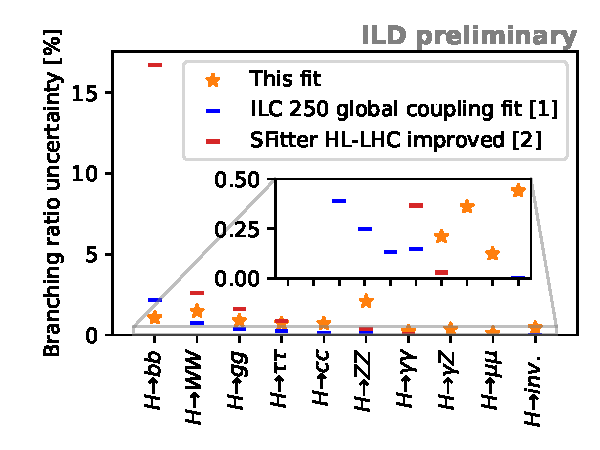
\includegraphics[width=\textwidth, keepaspectratio]
            {comparison_with_others}
    \end{column}
    \end{columns}
    \vspace{0.2\baselineskip}
    {\small
    [1] J.~Tian, K.~Fujii~\href{https://www.sciencedirect.com/science/article/pii/S2405601415006161}
        {\color{llblue} \textit{Measurement of Higgs boson couplings at the International Linear Collider}}.
    [2] SFitter~\href{https://inspirehep.net/literature/1209590}
        {\color{llblue} \textit{Measuring Higgs Couplings at a Linear Collider}}.
    }
    \end{frame}
